\documentclass[12pt,oneside]{book}

%%%%%%%%%%%%%%%%%%%%%%%%%%%%%%%%%%%%%%%%%%%%%%%%%%%%%%%%%%%%%%%%%%%%%%%%%%%%%%%%%%%%%%%%%%%%%%%%%%%
%                                                                                                 %
% The mathematical style of these documents follows                                               %
%                                                                                                 %
% A. Thompson and B.N. Taylor. The NIST Guide for the Use of the International System of Units.   %
%    NIST Special Publication 881, 2008.                                                          %
%                                                                                                 %
% http://www.nist.gov/pml/pubs/sp811/index.cfm                                                    %
%                                                                                                 %
%%%%%%%%%%%%%%%%%%%%%%%%%%%%%%%%%%%%%%%%%%%%%%%%%%%%%%%%%%%%%%%%%%%%%%%%%%%%%%%%%%%%%%%%%%%%%%%%%%%

% $Date: 2013-11-26 10:43:59 -0500 (Tue, 26 Nov 2013) $
% $Revision: 17538 $
% $Author: gforney $

%%%%%%%%%%%%%%%%%%%%%%%%%%%%%%%%%%%%%%%%%%%%%%%%%%%%%%%%%%%%%%%%%%%%%%%%%%%%%%%%%%%%%%%%%%%%%%%%%%%
%                                                                                                 %
% The mathematical style of these documents follows                                               %
%                                                                                                 %
% A. Thompson and B.N. Taylor. The NIST Guide for the Use of the International System of Units.   %
%    NIST Special Publication 881, 2008.                                                          %
%                                                                                                 %
% http://www.nist.gov/pml/pubs/sp811/index.cfm                                                    %
%                                                                                                 %
%%%%%%%%%%%%%%%%%%%%%%%%%%%%%%%%%%%%%%%%%%%%%%%%%%%%%%%%%%%%%%%%%%%%%%%%%%%%%%%%%%%%%%%%%%%%%%%%%%%

% Packages which force the use of better TeX coding
% Mostly from http://tex.stackexchange.com/q/19264
%%\RequirePackage[l2tabu, orthodox]{nag}
%%\usepackage{fixltx2e}
%\usepackage{isomath} % Disabled for the moment because it changes the syntax for bold and roman Greek math symbols
%%\usepackage[all,warning]{onlyamsmath}
%\usepackage{strict} % Commented out for now because it is uncommon. A copy of style.sty is in Manuals/LaTeX_Style_Files/.

\usepackage{times,mathptmx}
\usepackage[pdftex]{graphicx}
\usepackage{tabularx,ragged2e,booktabs,caption}
\usepackage{multirow}
\usepackage{pdfsync}
\usepackage{tikz}
\usepackage{pgfplots}
%\pgfplotsset{compat=1.7}
\usepackage{tocloft}
\usepackage{color}
\usepackage{amsmath}
\definecolor{linknavy}{rgb}{0,0,0.50196}
\definecolor{linkred}{rgb}{1,0,0}
\definecolor{linkblue}{rgb}{0,0,1}
\usepackage{float}
\usepackage{caption}
\usepackage{graphpap}
\usepackage{rotating}
\usepackage{graphicx}
\usepackage{geometry}
\usepackage{relsize}
\usepackage{longtable}
\usepackage{lscape}
\usepackage{amssymb}
\usepackage{makeidx} % Create index at end of document
\usepackage[nottoc,notlof,notlot]{tocbibind} % Put the bibliography and index in the ToC
\usepackage{lastpage} % Automatic last page number reference.
\usepackage[T1]{fontenc}
\usepackage{enumerate}
\usepackage{upquote}
\usepackage{moreverb}
\usepackage{xfrac}
\usepackage{cite}

\newcommand{\nopart}{\expandafter\def\csname Parent-1\endcsname{}} % To fix table of contents in pdf.
\newcommand{\ct}{\tt\small} % eventually will be deprecated due to http://www.tex.ac.uk/cgi-bin/texfaq2html?label=2letterfontcmd
\newcommand{\textct}[1]{\texttt{\small #1}}

\usepackage{tocstyle} % Fix table of contents sections from overlapping section titles
\usetocstyle{standard}
\usepackage{siunitx}
\sisetup{
    detect-all = true,
    input-decimal-markers = {.},
    input-ignore = {,},
    inter-unit-product = \ensuremath{{}\cdot{}},
    multi-part-units = repeat,
    number-unit-product = \text{~},
    per-mode = fraction,
    separate-uncertainty = true,
}

\usepackage{listings}
\usepackage{textcomp}
\definecolor{lbcolor}{rgb}{0.96,0.96,0.96}
\lstset{
    %backgroundcolor=\color{lbcolor},
    tabsize=4,
    rulecolor=,
    language=Fortran,
        basicstyle=\footnotesize\ttfamily,
        upquote=true,
        aboveskip={\baselineskip},
        belowskip={\baselineskip},
        columns=fixed,
        extendedchars=true,
        breaklines=true,
        breakatwhitespace=true,
        frame=none,
        showtabs=false,
        showspaces=false,
        showstringspaces=false,
        identifierstyle=\ttfamily,
        keywordstyle=\color[rgb]{0,0,0},
        commentstyle=\color[rgb]{0,0,0},
        stringstyle=\color[rgb]{0,0,0},
}

\usepackage[pdftex,
        colorlinks=true,
        urlcolor=linkblue,     % \href{...}{...} external (URL)
        citecolor=linkred,     % citation number colors
        linkcolor=linknavy,    % \ref{...} and \pageref{...}
        pdfproducer={pdflatex},
        pdfpagemode=UseNone,
        bookmarksopen=true,
        plainpages=false,
        verbose]{hyperref}

% The Following commented code makes the ``Draft'' watermark on each page.
%\usepackage{eso-pic}
%\usepackage{type1cm}
%\makeatletter
%   \AddToShipoutPicture{
%     \setlength{\@tempdimb}{.5\paperwidth}
%     \setlength{\@tempdimc}{.5\paperheight}
%     \setlength{\unitlength}{1pt}
%     \put(\strip@pt\@tempdimb,\strip@pt\@tempdimc){
%     \makebox(0,0){\rotatebox{45}{\textcolor[gray]{0.75}{\fontsize{8cm}\selectfont{RC6}}}}}
% }
%\makeatother

\setlength{\textwidth}{6.5in}
\setlength{\textheight}{9.0in}
\setlength{\topmargin}{0.in}
\setlength{\headheight}{0.pt}
\setlength{\headsep}{0.in}
\setlength{\parindent}{0.25in}
\setlength{\oddsidemargin}{0.0in}
\setlength{\evensidemargin}{0.0in}
\setlength{\leftmargini}{\parindent} % Controls the indenting of the "bullets" in a list
\setlength{\cftsecnumwidth}{0.45in}
\setlength{\cftsubsecnumwidth}{0.5in}
\setlength{\cftfignumwidth}{0.45in}
\setlength{\cfttabnumwidth}{0.45in}

\newcommand{\titlesigs}
{
\small
\flushright{U.S. Department of Commerce \\
{\em Penny Pritzker, Secretary} \\
\hspace{1in} \\
National Institute of Standards and Technology \\
{\em Willie May, Under Secretary of Commerce for Standards and Technology and Acting Director} }
}

% commands to use for "official" cover and title pages
% see smokeview verification guide to see how they are used

\newcommand{\headerA}[1]{
\flushright{
\fontsize{20}{24}\selectfont
\bf{NIST Special Publication #1}}
}

\newcommand{\headerB}[1]{
\flushright{
\fontsize{28}{33.6}\selectfont
\bf{#1}
}
}

\newcommand{\headerC}[1]{
\vspace{.5in}
\flushright{\fontsize{14}{16.8}\selectfont
#1}
}

\frenchspacing

\newcommand{\dod}[2]{\frac{\partial #1}{\partial #2}}
\newcommand{\DoD}[2]{\frac{\mathrm{D} #1}{\mathrm{D} #2}}
\newcommand{\dsods}[2]{\frac{\partial^2 #1}{\partial #2^2}}
\renewcommand{\d}{\,\mathrm{d}}
\newcommand{\dx}{\delta x}
\newcommand{\dy}{\delta y}
\newcommand{\dz}{\delta z}
\newcommand{\degF}{$^\circ$F}
\newcommand{\degC}{$^\circ$C}
\newcommand{\x}{x}
\newcommand{\y}{y}
\newcommand{\z}{z}
\newcommand{\dt}{\delta t}
\newcommand{\dn}{\delta n}
\newcommand{\cH}{H}
\newcommand{\hu}{u}
\newcommand{\hv}{v}
\newcommand{\hw}{w}
\newcommand{\la}{\lambda}
\newcommand{\bO}{{\Omega}}
\newcommand{\bo}{{\mathbf{\omega}}}
\newcommand{\btau}{\mathbf{\tau}}
\newcommand{\bdelta}{{\mathbf{\delta}}}
\newcommand{\sumyw}{\sum (Y_\alpha/W_\alpha)}
\newcommand{\oW}{\overline{W}}
\newcommand{\om}{\ensuremath{\omega}}
\newcommand{\omx}{\omega_x}
\newcommand{\omy}{\omega_y}
\newcommand{\omz}{\omega_z}
\newcommand{\erf}{\hbox{erf}}
\newcommand{\erfc}{\hbox{erfc}}
\newcommand{\bF}{{\mathbf{F}}}
\newcommand{\bG}{{\mathbf{G}}}
\newcommand{\bof}{{\mathbf{f}}}
\newcommand{\bq}{{\mathbf{q}}}
\newcommand{\br}{{\mathbf{r}}}
\newcommand{\bu}{{\mathbf{u}}}
\newcommand{\bx}{{\mathbf{x}}}
\newcommand{\bk}{{\mathbf{k}}}
\newcommand{\bv}{{\mathbf{v}}}
\newcommand{\bg}{{\mathbf{g}}}
\newcommand{\bn}{{\mathbf{n}}}
\newcommand{\bS}{{\mathbf{S}}}
\newcommand{\bW}{\overline{W}}
\newcommand{\dS}{d{\mathbf{S}}}
\newcommand{\bs}{{\mathbf{s}}}
\newcommand{\bI}{{\mathbf{I}}}
\newcommand{\hp}{H}
\newcommand{\trho}{\tilde{\rho}}
\newcommand{\dph}{{\delta\phi}}
\newcommand{\dth}{{\delta\theta}}
\newcommand{\tp}{\tilde{p}}
\newcommand{\bp}{\overline{p}}
\newcommand{\dQ}{\dot{Q}}
\newcommand{\dq}{\dot{q}}
\newcommand{\dbq}{\dot{\mathbf{q}}}
\newcommand{\dm}{\dot{m}}
\newcommand{\ha}{\frac{1}{2}}
\newcommand{\ft}{\frac{4}{3}}
\newcommand{\ot}{\frac{1}{3}}
\newcommand{\fofi}{\frac{4}{5}}
\newcommand{\of}{\frac{1}{4}}
\newcommand{\twth}{\frac{2}{3}}
\newcommand{\R}{R}
\newcommand{\be}{\begin{equation}}
\newcommand{\ee}{\end{equation}}
\newcommand{\RE}{\hbox{Re}}
\newcommand{\LE}{\hbox{Le}}
\newcommand{\PR}{\hbox{Pr}}
\newcommand{\PE}{\hbox{Pe}}
\newcommand{\NU}{\hbox{Nu}}
\newcommand{\SC}{\hbox{Sc}}
\newcommand{\SH}{\hbox{Sh}}
\newcommand{\WE}{\hbox{We}}
\newcommand{\COTWO}{\text{\tiny \hbox{CO}$_2$}}
\newcommand{\HTWOO}{\text{\tiny \hbox{H}$_2$\hbox{O}}}
\newcommand{\OTWO}{\text{\tiny \hbox{O}$_2$}}
\newcommand{\NTWO}{\text{\tiny \hbox{N}$_2$}}
\newcommand{\CO}{\text{\tiny \hbox{CO}}}
\newcommand{\F}{\text{\tiny \hbox{F}}}
\newcommand{\C}{\text{\tiny \hbox{C}}}
\newcommand{\Hy}{\text{\tiny \hbox{H}}}
\newcommand{\So}{\text{\tiny \hbox{S}}}
\newcommand{\M}{\text{\tiny \hbox{M}}}
\newcommand{\xx}{\text{\tiny \hbox{x}}}
\newcommand{\yy}{\text{\tiny \hbox{y}}}
\newcommand{\zz}{\text{\tiny \hbox{z}}}
\newcommand{\smvlines}{115~000}

\newcommand{\calH}{\mathcal{H}}
\newcommand{\calR}{\mathcal{R}}

\newcommand{\dif}{\mathrm{d}}
\newcommand{\Div}{\nabla\cdot}
\newcommand{\D}{\mbox{D}}
\newcommand{\mhalf}{\mbox{$\frac{1}{2}$}}
\newcommand{\thalf}{\mbox{\tiny $\frac{1}{2}$}}
\newcommand{\tripleprime}{{\prime\prime\prime}}
\newcommand{\ppp}{{\prime\prime\prime}}
\newcommand{\pp}{{\prime\prime}}

\newcommand{\superscript}[1]{\ensuremath{^{\textrm{\tiny #1}}}}
\newcommand{\subscript}[1]{\ensuremath{_{\textrm{\tiny #1}}}}

\newcommand{\rb}[1]{\raisebox{1.5ex}[0pt]{#1}}

\newcommand{\Ra}{$\Rightarrow$}
\newcommand{\hhref}[1]{\href{#1}{{\tt #1}}}
\newcommand{\fdsinput}[1]{{\scriptsize\verbatiminput{../../Verification/Visualization/#1}}}

\definecolor{AQUAMARINE}{rgb}{0.49804,1.00000,0.83137}
\definecolor{ANTIQUE WHITE}{rgb}{0.98039,0.92157,0.84314}
\definecolor{BEIGE}{rgb}{0.96078,0.96078,0.86275}
\definecolor{BLACK}{rgb}{0.00000,0.00000,0.00000}
\definecolor{BLUE}{rgb}{0.00000,0.00000,1.00000}
\definecolor{BLUE VIOLET}{rgb}{0.54118,0.16863,0.88627}
\definecolor{BRICK}{rgb}{0.61176,0.40000,0.12157}
\definecolor{BROWN}{rgb}{0.64706,0.16471,0.16471}
\definecolor{BURNT SIENNA}{rgb}{0.54118,0.21176,0.05882}
\definecolor{BURNT UMBER}{rgb}{0.54118,0.20000,0.14118}
\definecolor{CADET BLUE}{rgb}{0.37255,0.61961,0.62745}
\definecolor{CHOCOLATE}{rgb}{0.82353,0.41176,0.11765}
\definecolor{COBALT}{rgb}{0.23922,0.34902,0.67059}
\definecolor{CORAL}{rgb}{1.00000,0.49804,0.31373}
\definecolor{CYAN}{rgb}{0.00000,1.00000,1.00000}
\definecolor{DIMGRAY }{rgb}{0.41176,0.41176,0.41176}
\definecolor{EMERALD GREEN}{rgb}{0.00000,0.78824,0.34118}
\definecolor{FIREBRICK}{rgb}{0.69804,0.13333,0.13333}
\definecolor{FLESH}{rgb}{1.00000,0.49020,0.25098}
\definecolor{FOREST GREEN}{rgb}{0.13333,0.54510,0.13333}
\definecolor{GOLD }{rgb}{1.00000,0.84314,0.00000}
\definecolor{GOLDENROD}{rgb}{0.85490,0.64706,0.12549}
\definecolor{GRAY}{rgb}{0.50196,0.50196,0.50196}
\definecolor{GREEN}{rgb}{0.00000,1.00000,0.00000}
\definecolor{GREEN YELLOW}{rgb}{0.67843,1.00000,0.18431}
\definecolor{HONEYDEW}{rgb}{0.94118,1.00000,0.94118}
\definecolor{HOT PINK}{rgb}{1.00000,0.41176,0.70588}
\definecolor{INDIAN RED}{rgb}{0.80392,0.36078,0.36078}
\definecolor{INDIGO}{rgb}{0.29412,0.00000,0.50980}
\definecolor{IVORY}{rgb}{1.00000,1.00000,0.94118}
\definecolor{IVORY BLACK}{rgb}{0.16078,0.14118,0.12941}
\definecolor{KELLY GREEN}{rgb}{0.00000,0.50196,0.00000}
\definecolor{KHAKI}{rgb}{0.94118,0.90196,0.54902}
\definecolor{LAVENDER}{rgb}{0.90196,0.90196,0.98039}
\definecolor{LIME GREEN}{rgb}{0.19608,0.80392,0.19608}
\definecolor{MAGENTA}{rgb}{1.00000,0.00000,1.00000}
\definecolor{MAROON}{rgb}{0.50196,0.00000,0.00000}
\definecolor{MELON}{rgb}{0.89020,0.65882,0.41176}
\definecolor{MIDNIGHT BLUE}{rgb}{0.09804,0.09804,0.43922}
\definecolor{MINT}{rgb}{0.74118,0.98824,0.78824}
\definecolor{NAVY}{rgb}{0.00000,0.00000,0.50196}
\definecolor{OLIVE}{rgb}{0.50196,0.50196,0.00000}
\definecolor{OLIVE DRAB}{rgb}{0.41961,0.55686,0.13725}
\definecolor{ORANGE}{rgb}{1.00000,0.50196,0.00000}
\definecolor{ORANGE RED}{rgb}{1.00000,0.27059,0.00000}
\definecolor{ORCHID}{rgb}{0.85490,0.43922,0.83922}
\definecolor{PINK}{rgb}{1.00000,0.75294,0.79608}
\definecolor{POWDER BLUE}{rgb}{0.69020,0.87843,0.90196}
\definecolor{PURPLE}{rgb}{0.50196,0.00000,0.50196}
\definecolor{RASPBERRY}{rgb}{0.52941,0.14902,0.34118}
\definecolor{RED}{rgb}{1.00000,0.00000,0.00000}
\definecolor{ROYAL BLUE}{rgb}{0.25490,0.41176,0.88235}
\definecolor{SALMON}{rgb}{0.98039,0.50196,0.44706}
\definecolor{SANDY BROWN}{rgb}{0.95686,0.64314,0.37647}
\definecolor{SEA GREEN}{rgb}{0.32941,1.00000,0.62353}
\definecolor{SEPIA}{rgb}{0.36863,0.14902,0.07059}
\definecolor{SIENNA}{rgb}{0.62745,0.32157,0.17647}
\definecolor{SILVER}{rgb}{0.75294,0.75294,0.75294}
\definecolor{SKY BLUE}{rgb}{0.52941,0.80784,0.92157}
\definecolor{SLATEBLUE}{rgb}{0.41569,0.35294,0.80392}
\definecolor{SLATE GRAY}{rgb}{0.43922,0.50196,0.56471}
\definecolor{SPRING GREEN}{rgb}{0.00000,1.00000,0.49804}
\definecolor{STEEL BLUE}{rgb}{0.27451,0.50980,0.70588}
\definecolor{TAN}{rgb}{0.82353,0.70588,0.54902}
\definecolor{TEAL}{rgb}{0.00000,0.50196,0.50196}
\definecolor{THISTLE}{rgb}{0.84706,0.74902,0.84706}
\definecolor{TOMATO }{rgb}{1.00000,0.38824,0.27843}
\definecolor{TURQUOISE}{rgb}{0.25098,0.87843,0.81569}
\definecolor{VIOLET}{rgb}{0.93333,0.50980,0.93333}
\definecolor{VIOLET RED}{rgb}{0.81569,0.12549,0.56471}
\definecolor{WHITE}{rgb}{1.00000,1.00000,1.00000}
\definecolor{YELLOW}{rgb}{1.00000,1.00000,0.00000}

\pgfplotsset{
	colormap={blackwhite}{[5pt]
		rgb255(0pt)=(0,0,255); 
		rgb255(100pt)=(0,255,255); 
		rgb255(200pt)=(0,255,0); 
		rgb255(300pt)=(255,255,0); 
		rgb255(400pt)=(255,0,0)
	},
} % defines smokeview colorbar


\floatstyle{boxed}
\newfloat{notebox}{H}{lon}
\newfloat{warning}{H}{low}

% Set default longtable alignment
\setlength\LTleft{0pt}
\setlength\LTright{0pt}


% Rename chapter headings
\renewcommand{\chaptername}{Section}
\renewcommand{\bibname}{References}

% Math shortcuts
\renewcommand{\sb}[1]{_\mathrm{#1}}
\renewcommand{\C}{\mbox{C}}
\renewcommand{\H}{\mbox{H}}
\renewcommand{\O}{\mbox{O}}
\newcommand{\N}{\mbox{N}}

% Center all figures
\makeatletter
\g@addto@macro\@floatboxreset\centering
\makeatother

% Extra packages
\usepackage{xfrac}

\begin{document}

\bibliographystyle{unsrt}
\pagestyle{empty}

\begin{minipage}[t][9in][s]{6.25in}

\begin{flushright}
\fontsize{20}{24}\selectfont
\bf{NIST Technical Note XXXX}
\end{flushright}

\headerB{
Spartanburg Fire Tests \\
2013--2014 \\
}

\normalsize

\headerC{
{
\flushright{
Daniel Madrzykowski \\
Kristopher J. Overholt \\
Craig G. Weinschenk \\
Keith M. Stakes \\

\vspace*{2\baselineskip}

\begingroup
This publication is available free of charge from:
\hypersetup{urlcolor=black}
\href{http://dx.doi.org/10.6028/NIST.TN.XXXX}{http://dx.doi.org/10.6028/NIST.TN.XXXX}
\endgroup
}

\vfill

\flushright{


\includegraphics[width=2.in]{../../../Bibliography/nistident_flright_vec} \\[.3in]
}
}
}

\end{minipage}

\newpage
\hspace{5in}
\newpage

\frontmatter

\pagenumbering{roman}

\begin{minipage}[t][9in][s]{6.25in}

\begin{flushright}
\fontsize{20}{24}\selectfont
\bf{NIST Technical Note XXXX}
\end{flushright}

\headerB{
Spartanburg Fire Tests \\
2013--2014 \\
}

\headerC{
\flushright{
Daniel Madrzykowski \\
Kristopher J. Overholt \\
Craig G. Weinschenk \\
Keith M. Stakes \\
{\em Fire Research Division \\
Engineering Laboratory} \\

\vspace*{2\baselineskip}

\begingroup
This publication is available free of charge from:
\hypersetup{urlcolor=black}
\href{http://dx.doi.org/10.6028/NIST.TN.XXXX}{http://dx.doi.org/10.6028/NIST.TN.XXXX} \\
\endgroup

\vspace*{2\baselineskip}

August 2014}}

\vfill

\flushright{
\includegraphics[width=1in]{../../../Bibliography/doc} }

\titlesigs

\end{minipage}

\newpage

\begin{minipage}[t][9in][s]{6.25in}

\flushright{Certain commercial entities, equipment, or materials may be identified in this \\
document in order to describe an experimental procedure or concept adequately. \\
Such identification is not intended to imply recommendation or endorsement by the \\
National Institute of Standards and Technology, nor is it intended to imply that the \\
entities, materials, or equipment are necessarily the best available for the purpose. \\
}

\vspace{3in}

\large
\flushright{\bf National Institute of Standards and Technology Technical Note XXXX \\
Natl.~Inst.~Stand.~Technol.~Tech.~Note~XX, \pageref{LastPage} pages (August 2014) \\
CODEN: NTNOEF}

\vspace{0.2in}

\begingroup
{\bf This publication is available free of charge from:}
\hypersetup{urlcolor=black}
\href{http://dx.doi.org/10.6028/NIST.TN.XXXX}{\bf http://dx.doi.org/10.6028/NIST.TN.XXXX} \\
\endgroup

\vfill

\hspace{1in}

\end{minipage}

\newpage

\frontmatter

\pagestyle{plain}
\pagenumbering{roman}

\cleardoublepage
\phantomsection
\addcontentsline{toc}{chapter}{Contents}
\tableofcontents

\cleardoublepage
\phantomsection
\addcontentsline{toc}{chapter}{List of Figures}
\listoffigures

\cleardoublepage
\phantomsection
\addcontentsline{toc}{chapter}{List of Tables}
\listoftables

\chapter{List of Acronyms}

\begin{tabbing}
\hspace{1.5in} \= \\
FDS \> Fire Dynamics Simulator \\
HGL \> Hot Gas Layer \\
HRR \> Heat Release Rate \\
HRRPUA \> Heat Release Rate per Unit Area \\
NIST \> National Institute of Standards and Technology \\
\end{tabbing}

\mainmatter

\chapter{Introduction}
\label{chap:Introduction}

\chapter{Experimental Setup}
\label{chap:Experimental_Setup}

\section{Experimental Structure}
\label{sec:Experimental_Structure}

\section{Construction}
\label{sec:Construction}

\section{Instrumentation}
\label{sec:Instrumentation}

\begin{figure}[!ht]
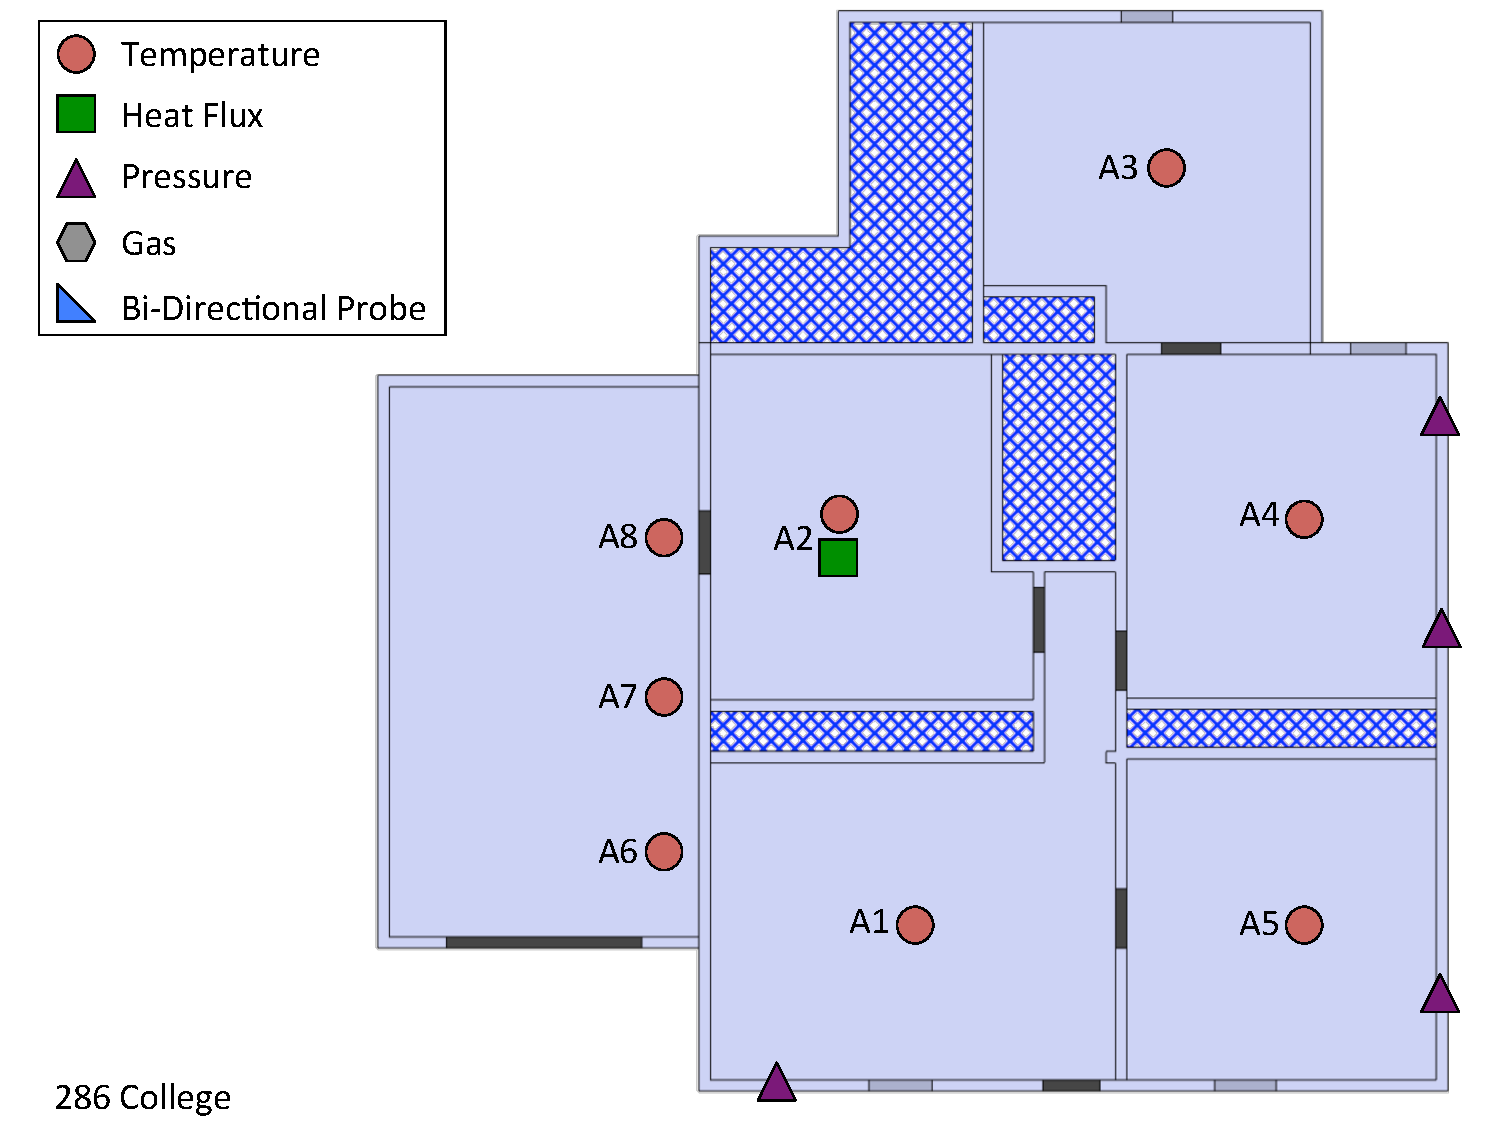
\includegraphics[width=6in]{../Figures/Instrumentation/286_College}
\caption{Instrumentation, 286 College}
\label{fig:Instrumentation_286_College}
\end{figure}

\begin{figure}[!ht]
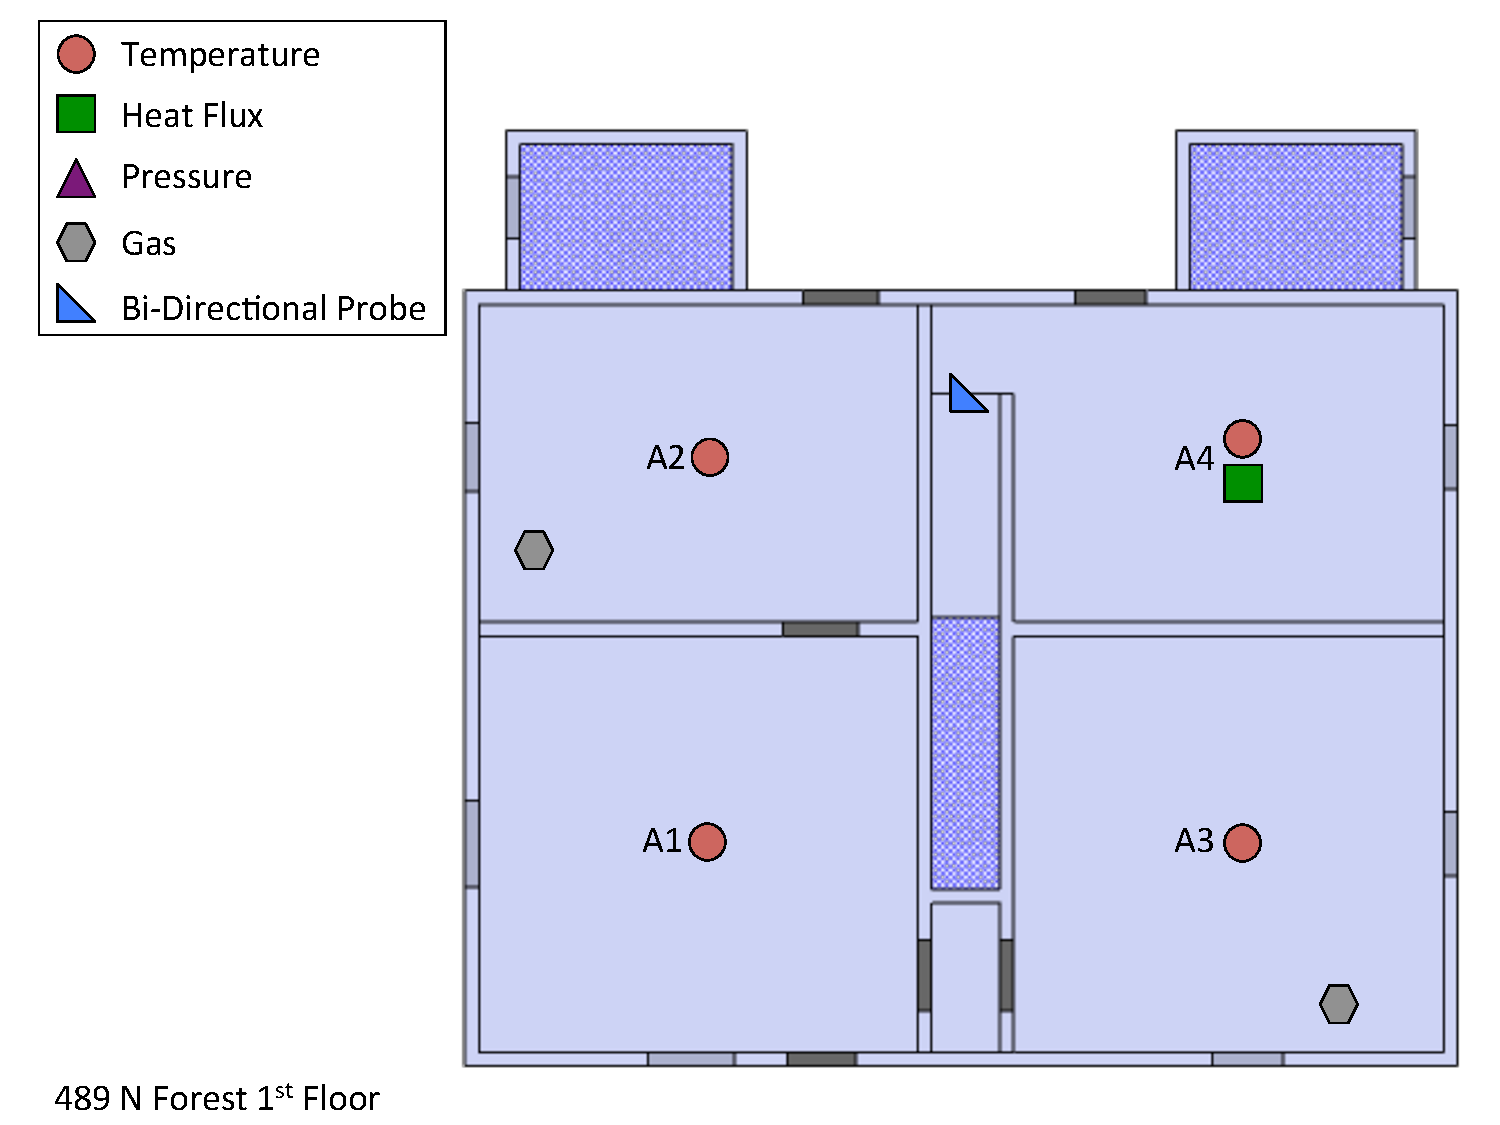
\includegraphics[width=6in]{../Figures/Instrumentation/489_N_Forest_1st_Floor}
\caption{Instrumentation, 489 N. Forest, first floor}
\label{fig:Instrumentation_489_N_Forest_1st_Floor}
\end{figure}

\begin{figure}[!ht]
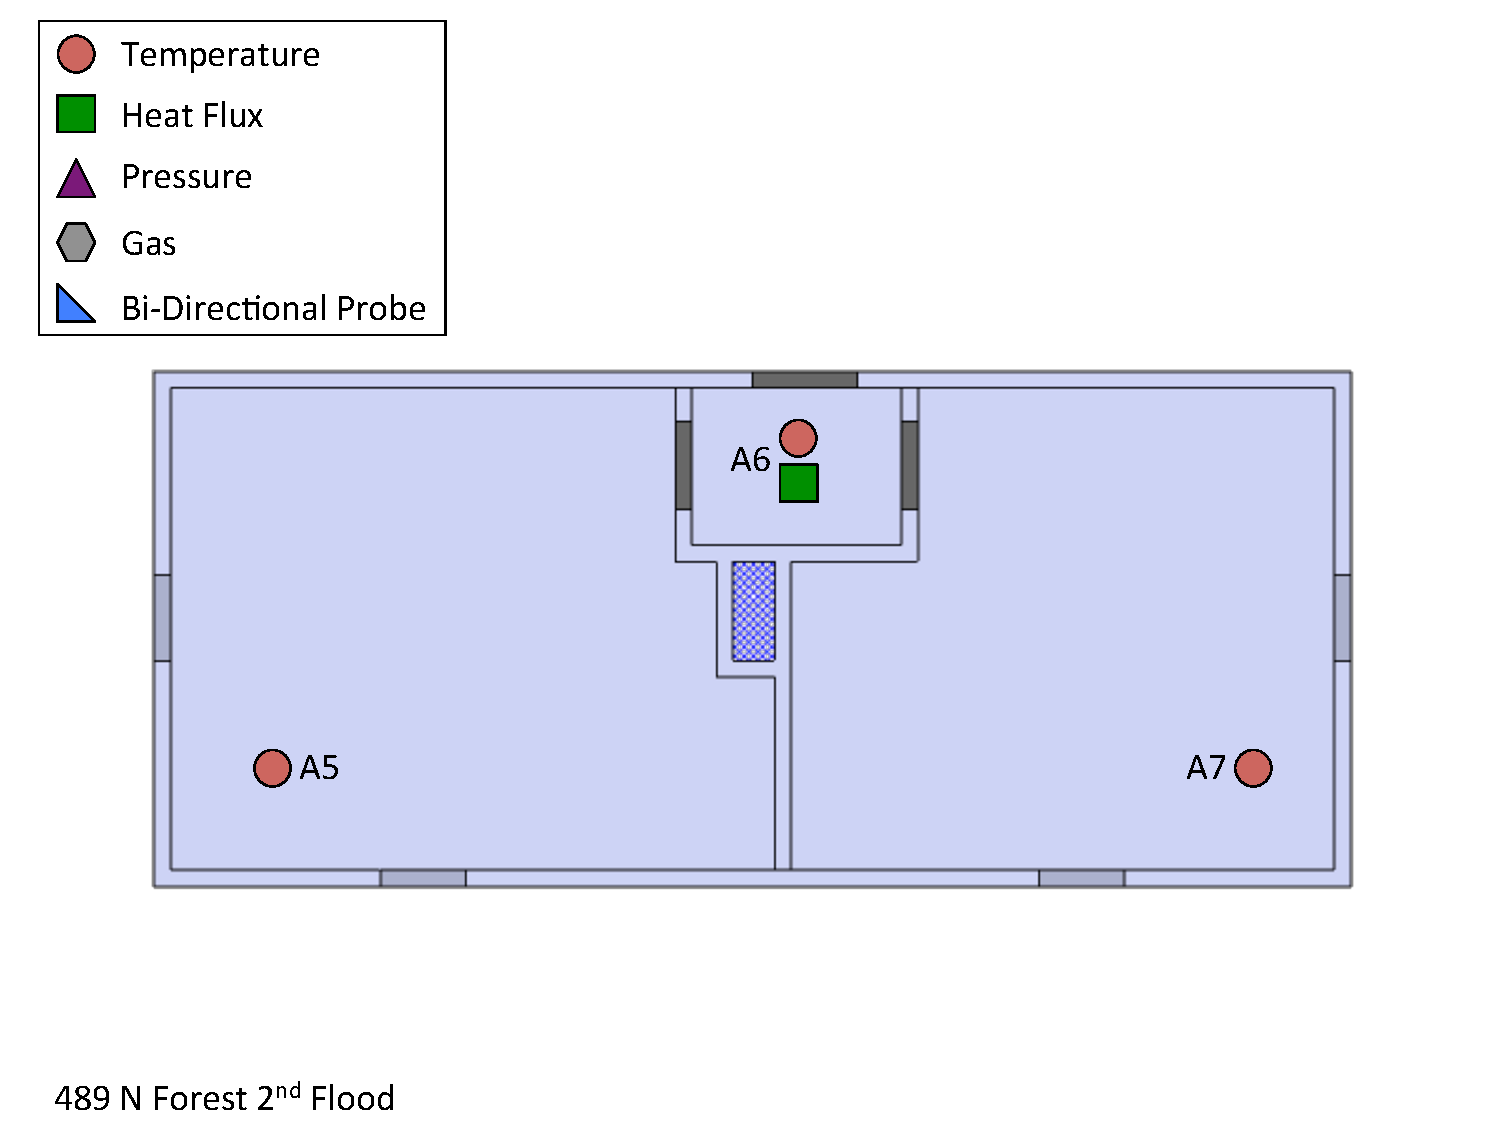
\includegraphics[width=6in]{../Figures/Instrumentation/489_N_Forest_2nd_Floor}
\caption{Instrumentation, 489 N. Forest, second floor}
\label{fig:Instrumentation_489_N_Forest_2nd_Floor}
\end{figure}

\begin{figure}[!ht]
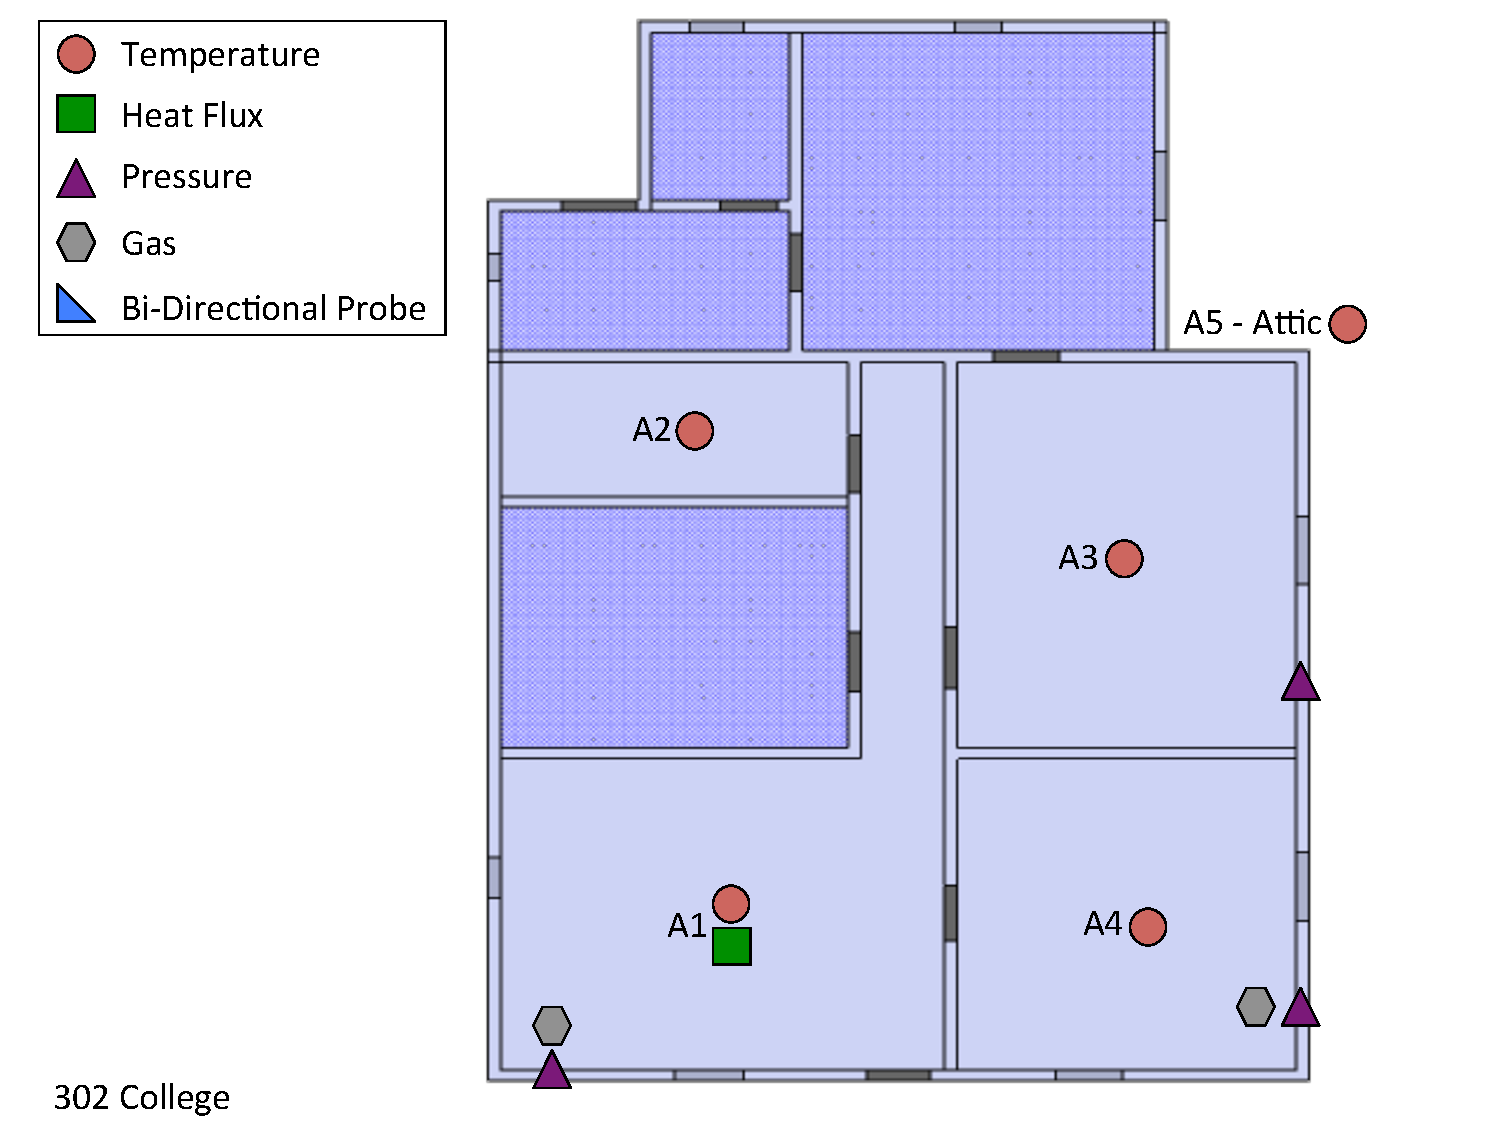
\includegraphics[width=6in]{../Figures/Instrumentation/302_College}
\caption{Instrumentation, 302 College}
\label{fig:Instrumentation_302_College}
\end{figure}

\begin{figure}[!ht]
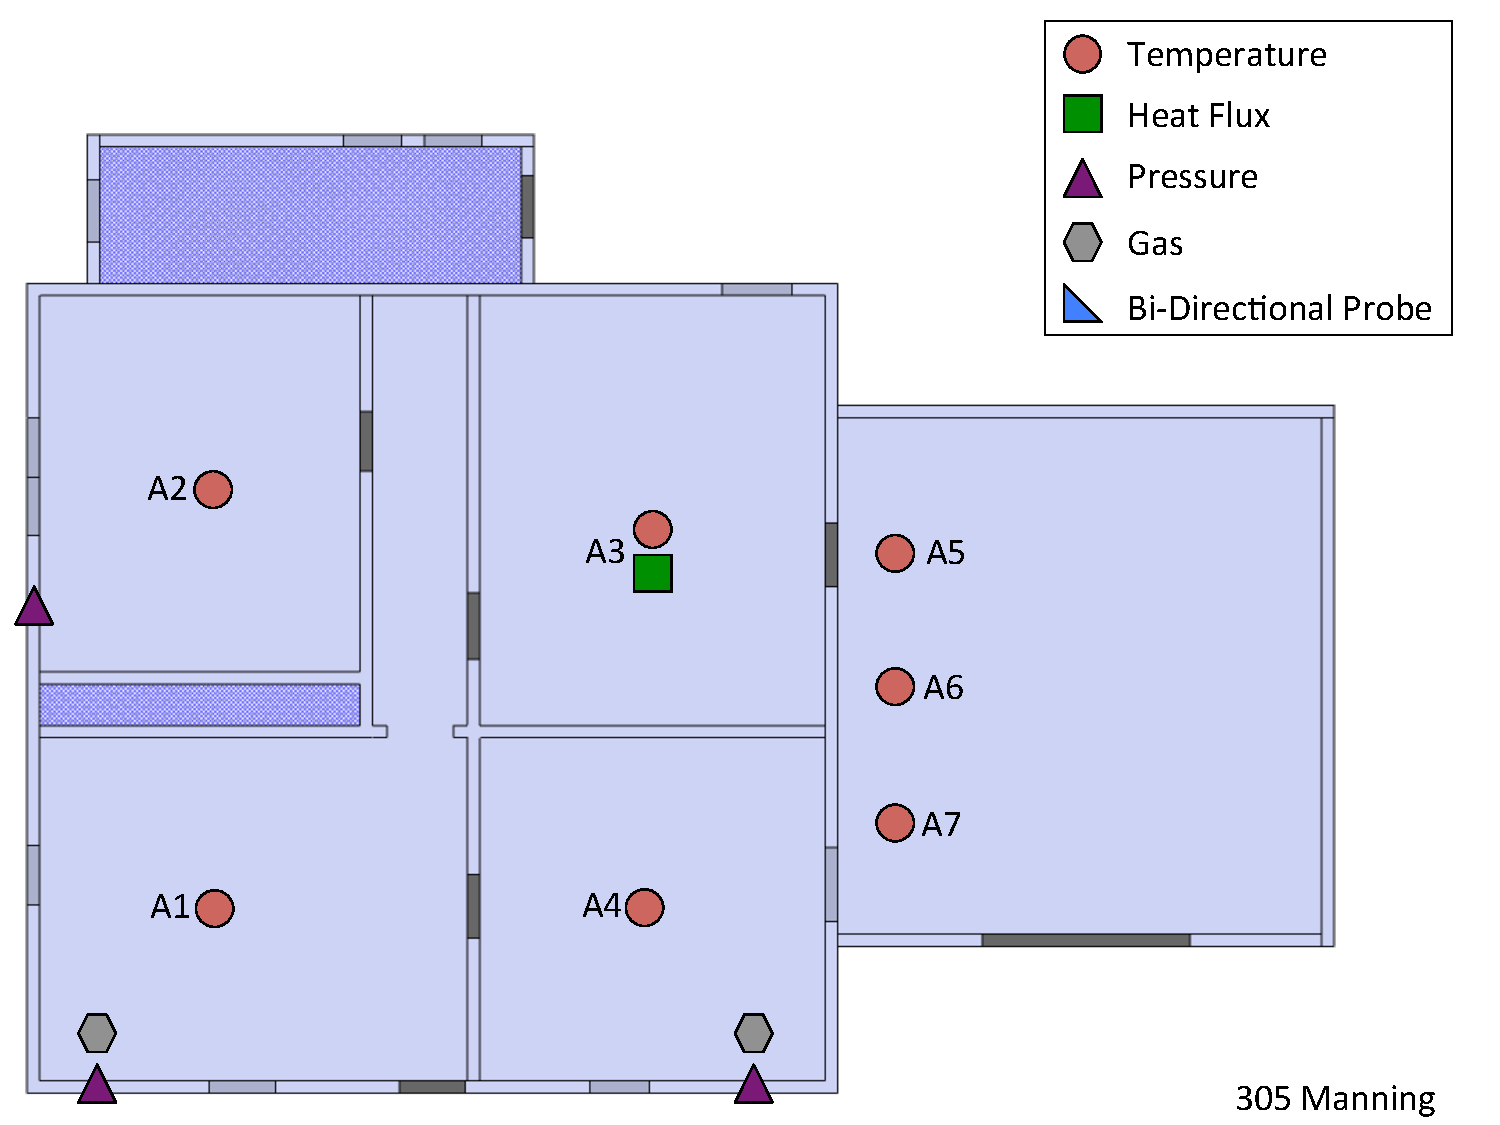
\includegraphics[width=6in]{../Figures/Instrumentation/305_Manning}
\caption{Instrumentation, 305 Manning}
\label{fig:Instrumentation_305_Manning}
\end{figure}

\begin{figure}[!ht]
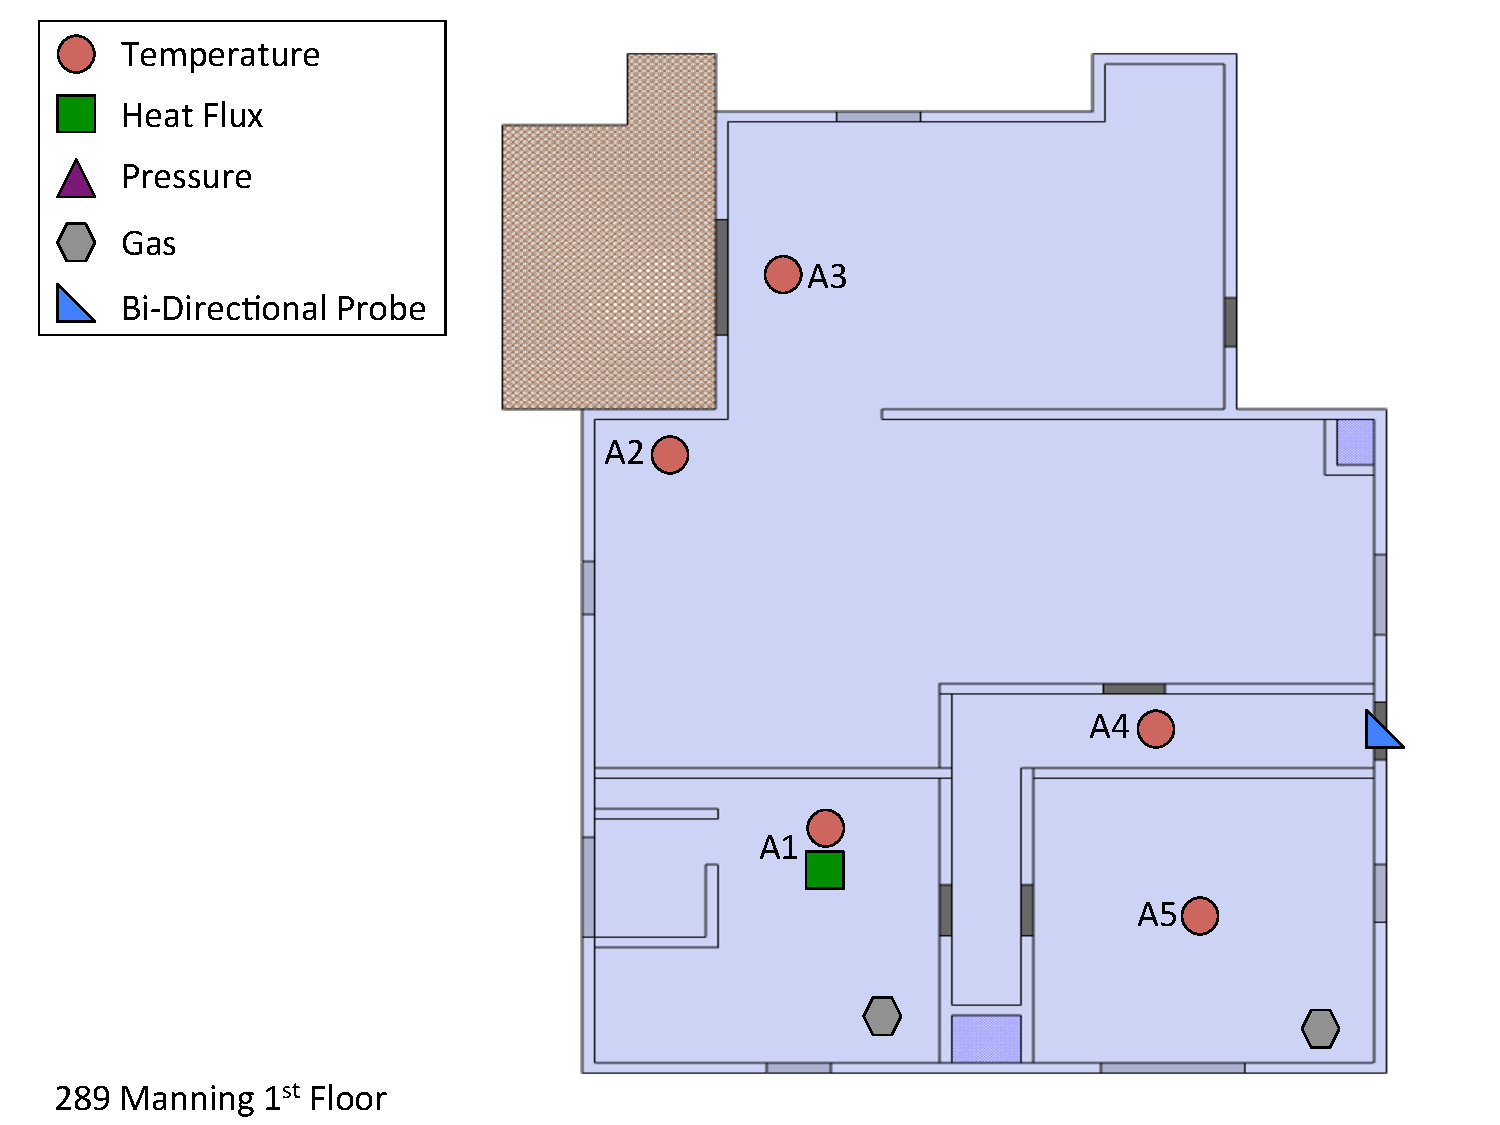
\includegraphics[width=6in]{../Figures/Instrumentation/289_Manning_1st_Floor}
\caption{Instrumentation, 289 Manning, first floor}
\label{fig:Instrumentation_289_Manning_1st_Floor}
\end{figure}

\begin{figure}[!ht]
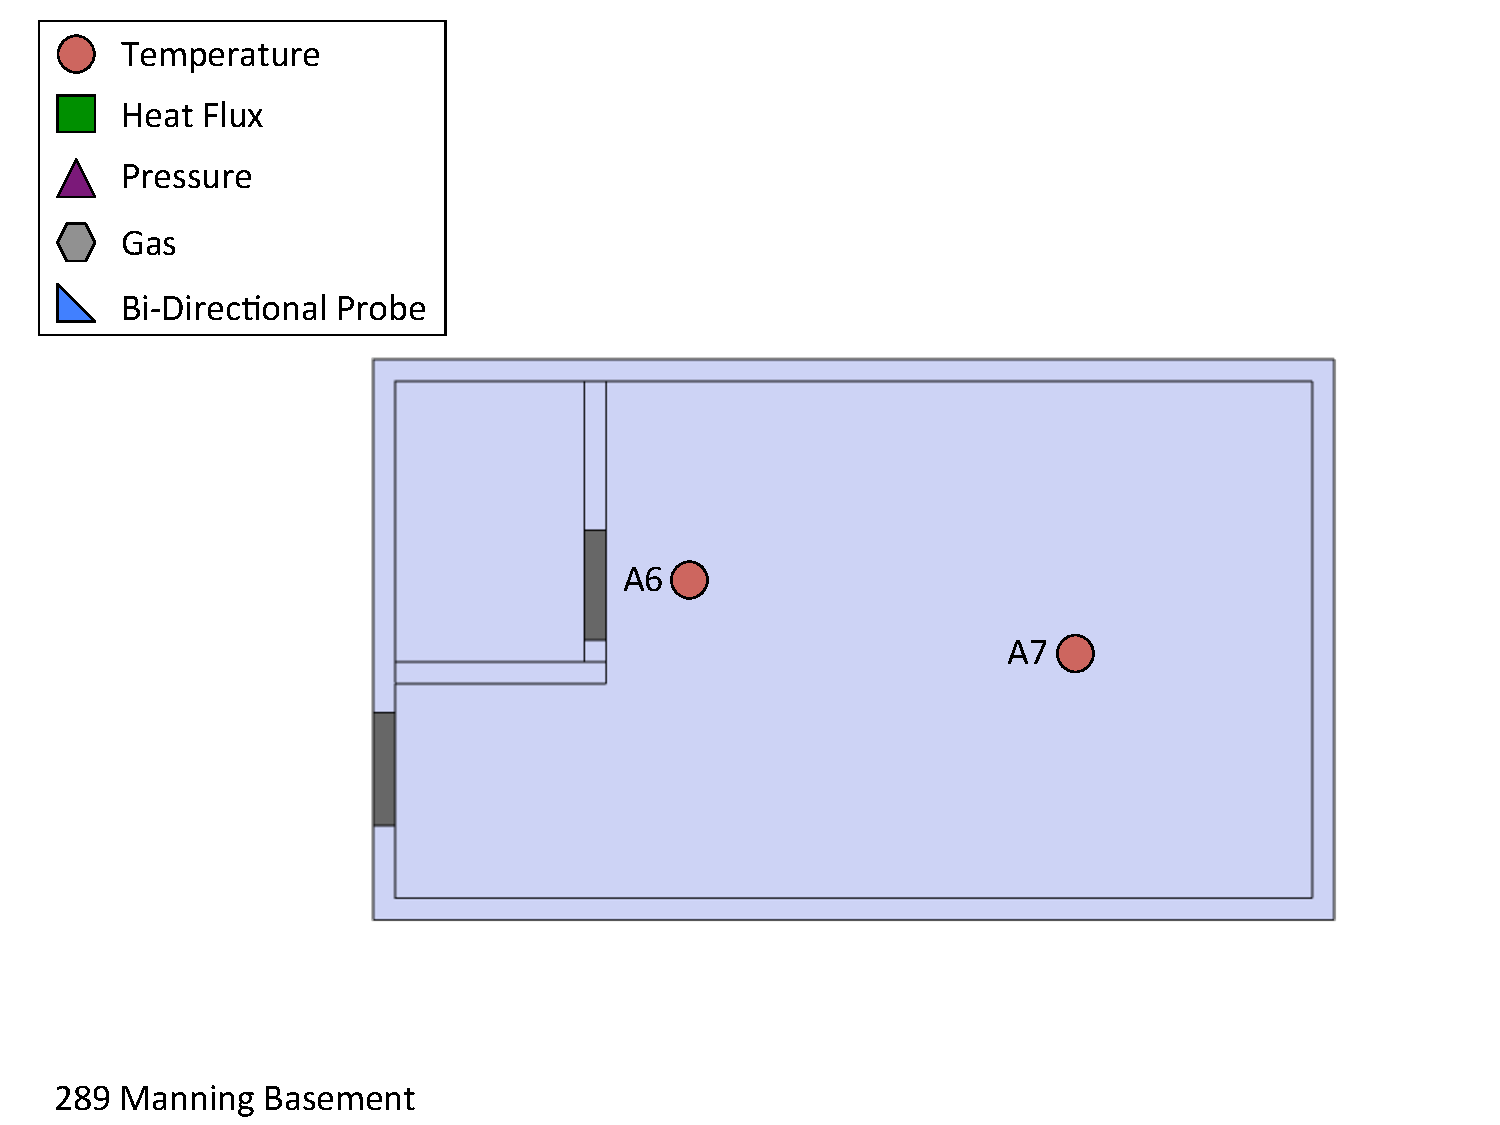
\includegraphics[width=6in]{../Figures/Instrumentation/289_Manning_Basement}
\caption{Instrumentation, 289 Manning, basement}
\label{fig:Instrumentation_289_Manning_basement}
\end{figure}


\clearpage


\section{Fuel Load}
\label{sec:Fuel_Load}

\begin{sidewaystable}[!ht]
\centering
\caption{Fuel masses}
\begin{tabular}{llcc}
\hline\noalign{\smallskip}
Item                         &  Material Description             &  Dimensions (m)            &  Mass (kg)  \\
\noalign{\smallskip}\hline\noalign{\smallskip}
% 3-seat Legacy Sofa         &  491 Brawley                      &  1.96 m x 0.86 m x 0.89 m  &  56.2 kg    \\
%   Cushion (left)           &  Cotton w/ inner springs          &                            &  4.06 kg    \\
%   Cushions (center)        &  Cotton w/ inner springs          &                            &  4.56 kg    \\
%   Cushions (rear)          &  Cotton w/ inner springs          &                            &  4.16 kg    \\
% 2-seat New Sofa            &  491 Brawley                      &  1.59 m x 0.91 m x 0.86 m  &  33.3 kg    \\
%   Cushion (seat)           &                                   &  0.56 m x 0.61 m x 0.14 m  &  1.6 kg     \\
%   Cushion (rear)           &  0.71 m at top, 0.58 m at bottom  &  Varies x 0.53 m x 0.20 m  &  2.0 kg     \\
3-seat Brown Sofa            &  302 College (front room)         &  2.24 m x 1.02 m x 0.91 m  &  61.0 kg    \\
2-seat Purple Stripe Sofa    &  302 College (front room)         &  1.57 m x 0.97 m x 0.86 m  &  82.0 kg    \\
3-seat Black Pine Leaf Sofa  &  302 College (front room)         &  2.08 m x 0.86 m x 0.86 m  &  51.0 kg    \\
Blue/Brown Chair             &  302 College (front room)         &  0.97 m x 0.81 m x 0.97 m  &  46.4 kg    \\
2-seat Floral Sofa           &  302 College (rear room)          &  1.68 m x 0.91 m x 0.91 m  &  34.5 kg    \\
2-seat Blue Plaid Sofa       &  302 College (rear room)          &  1.63 m x 0.97 m x 0.91 m  &  39.8 kg    \\
3-seat Yellow Sofa           &  302 College (rear room)          &  2.13 m x 0.91 m x 0.71 m  &  48.3 kg    \\
3-seat Floral Sofa           &  302 College (rear room)          &  2.29 m x 0.91 m x 0.91 m  &  48.0 kg    \\
3-seat New Sofa              &  289 College (front room)         &  2.13 m x 0.91 m x 0.91 m  &  43.0 kg    \\
Blue Chair                   &  289 College (middle room)        &  0.91 m x 0.91 m x 0.91 m  &  25.3 kg    \\
3-seat Floral Sofa           &  289 College (sprinkler room)     &  2.24 m x 1.02 m x 1.02 m  &  81.2 kg    \\
Floral Chair                 &  289 College (sprinkler room)     &  1.02 m x 1.02 m x 1.02 m  &  36.3 kg    \\
\noalign{\smallskip}\hline
\end{tabular}
\label{tab:Fuel_Masses}
\end{sidewaystable}

\chapter{Results}
\label{chap:Results}


\clearpage


\chapter{Conclusions}
\label{chap:Conclusions}

\chapter{Acknowledgments}
\label{chap:Acknowledgments}

\bibliography{../../../Bibliography/FDS_refs,../../../Bibliography/FDS_general,references}

\appendix

\chapter{All Tests}

\section{214 Folsom Street}

The first test house was a single story, single family residential structure of type 5 construction addressed as 214 Folsom Street. The non-burn rooms had a limited-combustible finish comprised of either paper-covered gypsum board or a finished plaster board. The burn rooms had a combustible finish comprised of OSB sheets for wall linings. Two tests were conducted in this structure: 1) Living room fire with exterior attack and 2) Bedroom fire with exterior attack.

\subsection{Test 1: Living Room Fire}

Ignition begins on a modern-style sofa in the living room on the A/D corner of the structure with all doors and windows closed. The fire grew uninhibited and reach the vent-limited stage. Fire fighting crew ventilated the living room window on the D side of the structure.The fire was allowed to stabilize with the new ventilation opening. The fire fighting crew then applied water, via a straight stream flow, from the exterior into the D side window for suppression. After the exterior suppression, the front living room window on the A side of the structure was ventilated. Water was then applied from the exterior on the A side into the living room window for further suppression. The fire fighting crew then opened the front door and made entry to complete suppression.

\subsection{Test 2: Bedroom Fire}

The fire was ignited on a modern-style soda in the bedroom located near the B/C corner of the structure. The living room used during the previous burn was isolated from the remaining portion of the building for this test to not alter the results. The fire was allowed to grow uninhibited and reach the vent-limited stage. The fire self-vented the upper portion of the bedroom window on the B side of the structure. The fire fighting crew ventilated a window on the D side of the building in the adjacent room located near the C/D corner. The fire then self-vented the remaining portion of the window in the room of origin. The small window into the kitchen on the B side of the structure was then ventilated. Shortly thereafter, the fire fighting crew made an exterior attack via a narrow fog into the bedroom from the self-vented B side window.

\section{215 Folsom Street}

The second test house was a single story, single family residential structure of type 5 construction addressed as 215 Folsom Street. The non-burn rooms had a limited-combustible finish comprised of either paper-covered gypsum board or a finished plaster board. The burn rooms had a combustible finish comprised of OSB sheets for wall linings. Two tests were conducted in this structure: 1) Living room fire with exterior attack and 2) Bedroom fire with exterior attack.

\subsection{Test 1: Living Room Fire}

The fire was ignited in the front living room located near the A/B corner of the structure on a modern-style sofa. The fire grew uninhibited until reaching the ventilation-limited stage. While in the growth stage, the fire self-vented the living room window on the A side of the structure, near the A/B corner. After the fire fighting unit officer completed a 360 degree size-up of the structure, the front door was opened from the exterior. The living room window on the B side of the structure then self-vented as well. Shortly thereafter, the pressure from the fire compartment closed the front door. After a short period of time, the fire fighting crew re-opened the front door to the building. The fire fighting crew began an attack on the structure via a single smooth bore hose-line first knocking down the fire on the porch. The nozzle was then directed into the A side living room window and front doorway. The fire fighting crew then completed suppression and overhauled the porch area to complete mop-up procedures.

\subsection{Test 2: Bedroom Fire}

The fire was ignited in a rear bedroom near the C/D corner of the structure on a modern-style sofa. The C side window to the bedroom was half open. The C side window in the adjoining room also had a window in the half open position. The living room used during the previous burn was isolated from the remaining portion of the building for this test to not alter the results. The fire was allowed to grow uninhibited and reach the vent-limited stage. The fire then self-vented a portion of the bedroom window on the D side. Once the temperatures leveled off in the fire room, the fire fighting crew ventilated the remaining portion of the window in the adjoining room, also on the D side of the structure. As the fire continued to grow, the fire fighting crew ventilated the remaining portion of the bedroom window in the room of origin. The fire room reached flashover conditions. The fire fighting crew then applied water into the room of origin via a single hose-line with a narrow fog pattern until the fire was completely suppressed.

\section{218 Folsom Street}

The third test house was a single story, single family residential structure of type 5 construction addressed as 218 Folsom Street. The non-burn rooms had a limited-combustible finish comprised of either paper-covered gypsum board or a finished plaster board. The burn rooms had a combustible finish comprised of OSB sheets for wall linings. Two tests were conducted in this structure: 1) Bedroom fire with exterior attack and 2) Bedroom fire with exterior attack. 

\subsection{Test 1: Bedroom Fire}

The fire was ignited in a rear bedroom near the C/D corner of the structure on a modern-style mattress with foam padding atop. All doors and windows to the exterior of the structure were closed at the beginning of the test. The fire grew uninhibited until reaching the vent-limited stage. The officer of the fire fighting crew completed a 360 degree size-up of the structure to assess conditions. Shortly thereafter, the fire fighting crew ventilated the bedroom window on the D side of the building. The fire was allowed to stabilize given the new ventilation opening. The fire fighting crew then made an attack on the fire by flowing a single hand-line with a smooth bore nozzle into the room of origin through the D side window from the exterior.

\subsection{Test 2: Bedroom Fire}

Ignition occurred in a rear bedroom near the B/C corner of the structure on a modern-style couch. All doors and windows to the exterior of the structure were closed at the beginning of the test. The bedroom used during the previous burn was isolated from the remaining portion of the building for this test to not alter the results. The fire grew uninhibited until reaching the vent-limited stage. The officer of the fire fighting crew completed a 360 degree size-up and then the fire fighting crew ventilated the target room window on the B side of the building. This was the window to the adjoining room in the structure located near the A/B corner. The fire was allowed to stabilize given the new ventilation opening. The fire fighting crew then ventilated the bedroom window to the room of origin on the B side next. This was followed up by the fire fighting crew making an attack on the fire by flowing a single hand-line with a smooth bore nozzle into the room of origin through the B side window from the exterior.

\section{219 Folsom Street}

The next test house was a single story, single family residential structure of type 5 construction addressed as 219 Folsom Street. The non-burn rooms had a limited-combustible finish comprised of either paper-covered gypsum board or a finished plaster board. The burn rooms had a combustible finish comprised of OSB sheets for wall linings. Two tests were conducted in this structure: 1) Bedroom fire with exterior attack and 2) Living room fire with exterior attack.

\subsection{Test 1: Bedroom Fire}

Ignition occurred in a rear bedroom near the B/C corner of the structure on a modern-style mattress with foam padding. All doors and windows to the exterior of the structure were closed at the beginning of the test. The fire grew uninhibited until reaching the vent-limited stage. The front door to the structure was then opened by the fire fighting crew to simulate a crew making entry or a homeowner leaving the door open upon evacuation. The fire continued to grow uninhibited until the fire room reached flashover conditions. The fire fighting crew then ventilated the bedroom window on the B side of the structure in the room of origin. The fire was then allowed to stabilize given the new ventilation opening. An unmanned monitor nozzle connected to a single hose-line was placed inside the structure at the entry to the fire room. This was remotely activated to simulate a fire fighting crew making an interior attack on the seat of the fire. The water was flowed until the fire was suppressed. The fire fighting crew then completed the test by making entry to the structure to complete overhaul and mop-up procedures. 

\subsection{Test 2: Living Room Fire}

The fire was ignited in the front living room located near the A/D corner of the structure on a modern-style sofa. The bedroom used during the previous burn was isolated from the remaining portion of the building for this test to not alter the results. The window to the living room on the D side of the structure was half-opened at the start of the test. The fire grew uninhibited until reaching the ventilation-limited stage. The window on the D side in the adjacent room near the C/D corner of the structure was ventilated next. The upper portion of the A side living room window self-ventilated due to the fire. Shortly thereafter, the fire fighting crew ventilated the remaining portion of the D side living room window. Once the fire had self-ventilated the remaining portion of the A side living room window, it was allowed to stabilize. The fire fighting crew then conducted an exterior attack via the D side living room window with a single hose-line with a smooth bore nozzle. 

\section{225 Folsom Street}

 The fifth test house was a single story, single family residential structure of type 5 construction addressed as 225 Folsom Street. The non-burn rooms had a limited-combustible finish comprised of either paper-covered gypsum board or a finished plaster board. The burn rooms had a combustible finish comprised of OSB sheets for wall linings. One test was conducted in this structure comparing a legacy versus modern sofa with an exterior fire attack.
 
\subsection{Test 1: Legacy versus Modern Sofa}

Ignition points were located in two different rooms within the home. A legacy-style sofa was ignited in a rear bedroom of the structure near the C/D corner and a modern-style sofa was ignited in a front living room near the A/B corner approximately 6 minutes after the first ignition. The front door to the structure remained open during the test. Additionally, the D side window to the rear bedroom with the legacy-style sofa also remained open. The fires were allowed to grow uninhibited. The fires within the home became ventilation limited. The living room window on the B side of the structure self-vented, followed by the living room window on the A side of the structure. Once the fire grew in size and began burning the porch area, an exterior attack via a single hose-line with smooth bore nozzle was made through the front door and A side living room window. 

\section{226 Folsom Street}

The following series of tests were conducted in a single story, single family residential structure of type 5 construction addressed as 226 Folsom Street. The non-burn rooms had a limited-combustible finish comprised of either paper-covered gypsum board or a finished plaster board. The burns rooms had a combustible finish comprised of OSB sheets for wall linings. Three tests were conducted in this structure: 1) Wastebasket fire with sprinkler activation, 2) Bedroom fire with exterior attack, and 3) Living room fire with exterior attack. 

\subsection{Test 1: Wastebasket Fire with Sprinkler}

This fire was ignited in a small wastebasket located between a bed with modern-style mattress and a wooden nightstand in the bedroom of the home near the A/D corner. The windows and door to the room were closed for the duration of the test. The fire grew uninhibited until the sprinkler activated suppressing the fire. Shortly thereafter, a fire fighting crew made entry to confirm extinguishment.

\subsection{Test 2: Bedroom Fire}

Ignition occurred on a modern-style mattress in a bedroom to the rear of the structure near the C/D corner. The bedroom window on side C of the structure is open during the test as is the interior bedroom doorway. The bedroom window on side D of the structure is closed at the beginning of the test. Fire growth was uninhibited. The fire in the room of origin grew until the D side window self-vented. The room of origin reached flashover conditions and the D side window became full exhaust. The adjoining bedroom window on the D side of the structure was vented by the fire fighting crew shortly thereafter. The fire fighting crew then conducted an exterior attack via a single hand-line with a smooth bore nozzle until the fire was extinguished. Another fire fighting crew made entry into the structure via the Side A door to confirm extinguishment and mop-up.

\subsection{Test 3: Living Room Fire}

The fire was ignited on a modern-style sofa in the living room near the A/B corner of the structure. The A side window to the living room, in addition to the A side front door, were open for the duration of the test. The fire was allowed to grow uninhibited until the fire building reached ventilation-limited conditions.

\section{286 College}

The first set of experiments were conducted in a single story residential structure with attached garage addressed as 286 College Street. The structure consisted of type 5 construction. The attached garage was added on to the B side of the structure for the purpose of these tests. The non-burn rooms had a limited-combustible finish comprised of either paper-covered gypsum board or a finished plaster board. The burn rooms had a combustible finish comprised of OSB sheets for wall linings. Three tests were conducted in this structure: 1) A living room fire with a residential sprinkler present, 2) An attached garage fire with exterior attack, and 3) A living room fire with door control.

\subsection{Test 1, Living room fire with sprinkler}

Test 1 consisted of a fire in the living room with residential sprinkler activation. Ignition occurred on a couch in the living room to the rear of the structure near the C/D corner. The fire was remotely ignited from the exterior of the structure. There was a residential sprinkler in the fire room. Other fire room furnishings included a sofa chair, two wooden end tables, a floor lamp, cloth window curtains, carpeted floor, and wooden paneling for wall linings. The fire grew uninhibited until the sprinkler activated and suppressed the bulk of the fire. A fire fighting crew made entry through side C for mop-up.

\begin{figure}[!ht]
\includegraphics[width=5in]{../Figures/Script_Figures/286_College_Test_1_TC_A3}
\caption{286 College, Test 1, Temperature TC\_A3}
\label{fig:286_College_Test_1_TC_A3}
\end{figure}

\begin{figure}[!ht]
\includegraphics[width=5in]{../Figures/Script_Figures/286_College_Test_1_TC_A4}
\caption{286 College, Test 1, Temperature TC\_A4}
\label{fig:286_College_Test_1_TC_A4}
\end{figure}

\begin{figure}[!ht]
\includegraphics[width=5in]{../Figures/Script_Figures/286_College_Test_1_TC_S_1}
\caption{286 College, Test 1, Temperature TC\_S\_1}
\label{fig:286_College_Test_1_TC_S_1}
\end{figure}


\clearpage


\subsection{Test 2, Garage fire, exterior attack}

Test 2 consisted of a fire in the attached garage with an exterior fire attack. Two separate ignition points were used, one of which was inside a car located in the garage and another was located on a couch to the rear of the garage. The couch simulated other fuel loads commonly found within a garage. Several wooden pallets were also placed in the garage for additional fuel. The fire was ignited remotely from the exterior of the garage. The door from the attached garage to the interior of the structure (kitchen area) remained closed for the duration of this test. The fire grew uninhibited in the garage until the space reached flashover conditions and became fully-involved. The fire was knocked down and suppressed from the exterior of the structure by a fire fighting crew with a single hand-line in a straight stream pattern. The front door on Side A of the structure was then opened to simulate a crew making entry. 

\begin{figure}[!ht]
\includegraphics[width=5in]{../Figures/Script_Figures/286_College_Test_2_TC_A1}
\caption{286 College, Test 2, Temperature TC\_A1}
\label{fig:286_College_Test_2_TC_A1}
\end{figure}

\begin{figure}[!ht]
\includegraphics[width=5in]{../Figures/Script_Figures/286_College_Test_2_TC_A2}
\caption{286 College, Test 2, Temperature TC\_A2}
\label{fig:286_College_Test_2_TC_A2}
\end{figure}

\begin{figure}[!ht]
\includegraphics[width=5in]{../Figures/Script_Figures/286_College_Test_2_TC_A6}
\caption{286 College, Test 2, Temperature TC\_A6}
\label{fig:286_College_Test_2_TC_A6}
\end{figure}

\begin{figure}[!ht]
\includegraphics[width=5in]{../Figures/Script_Figures/286_College_Test_2_TC_A7}
\caption{286 College, Test 2, Temperature TC\_A7}
\label{fig:286_College_Test_2_TC_A7}
\end{figure}

\begin{figure}[!ht]
\includegraphics[width=5in]{../Figures/Script_Figures/286_College_Test_2_TC_A8}
\caption{286 College, Test 2, Temperature TC\_A8}
\label{fig:286_College_Test_2_TC_A8}
\end{figure}

\begin{figure}[!ht]
\includegraphics[width=5in]{../Figures/Script_Figures/286_College_Test_2_HF}
\caption{286 College, Test 2, Heat Flux}
\label{fig:286_College_Test_2_HF}
\end{figure}

\begin{figure}[!ht]
\includegraphics[width=5in]{../Figures/Script_Figures/286_College_Test_2_P_S_1}
\caption{286 College, Test 2, Pressure}
\label{fig:286_College_Test_2_P_S_1}
\end{figure}


\clearpage


\subsection{Test 3, Living room fire}

Test 3 consisted of a fire in the living room located in the front of the structure near the A/B corner. The ignition point for this test was the corner of a modern-style couch and was performed remotely from the exterior of the structure. Other fuels present in the room were another modern-style sofa and a modern-style love seat. The fire room was lined with OSB paneling for additional fuel. The front side A door was in the open position for the start of the test. The target room, located adjacent to the fire room near the A/D corner, was separated by a closed hollow core wooden door. Once ignited, the fire grew uninhibited until the room approached flashover conditions. Prior to this, the front door to the room was closed. The fire was allowed to stabilize and then the front door was opened. The fire fighting crew made an attack from the exterior via a straight stream pattern from a single hand-line. The pattern was then switched to a narrow fog for further suppression. The fire fighting crew then made entry into the fire room for mop-up procedures.

\begin{figure}[!ht]
\includegraphics[width=5in]{../Figures/Script_Figures/286_College_Test_3_TC_A1}
\caption{286 College, Test 3, Temperature TC\_A1}
\label{fig:286_College_Test_3_TC_A1}
\end{figure}

\begin{figure}[!ht]
\includegraphics[width=5in]{../Figures/Script_Figures/286_College_Test_3_TC_A4}
\caption{286 College, Test 3, Temperature TC\_A4}
\label{fig:286_College_Test_3_TC_A4}
\end{figure}

\begin{figure}[!ht]
\includegraphics[width=5in]{../Figures/Script_Figures/286_College_Test_3_TC_A5}
\caption{286 College, Test 3, Temperature TC\_A5}
\label{fig:286_College_Test_3_TC_A5}
\end{figure}

\begin{figure}[!ht]
\includegraphics[width=5in]{../Figures/Script_Figures/286_College_Test_3_HF}
\caption{286 College, Test 3, Heat Flux}
\label{fig:286_College_Test_3_HF}
\end{figure}

\begin{figure}[!ht]
\includegraphics[width=5in]{../Figures/Script_Figures/286_College_Test_3_P_S_1}
\caption{286 College, Test 3, Pressure}
\label{fig:286_College_Test_3_P_S_1}
\end{figure}


\clearpage


\section{489 N. Forest}

The next set of experiments were conducted in a two story residential structure addressed as 489 North Forest Street. The structure consisted of type 5 construction. The non-burn rooms had a limited-combustible finish comprised of either paper-covered gypsum board or a finished plaster board. The burn rooms had a combustible finish comprised of OSB sheets for wall linings.

\subsection{Test 1, Living room fire}



\begin{figure}[!ht]
\includegraphics[width=5in]{../Figures/Script_Figures/489_N_Forest_Test_1_TC_A1}
\caption{489 N. Forest, Test 1, Temperature TC\_A1}
\label{fig:489_N_Forest_Test_1_TC_A1}
\end{figure}

\begin{figure}[!ht]
\includegraphics[width=5in]{../Figures/Script_Figures/489_N_Forest_Test_1_TC_A2}
\caption{489 N. Forest, Test 1, Temperature TC\_A2}
\label{fig:489_N_Forest_Test_1_TC_A2}
\end{figure}

\begin{figure}[!ht]
\includegraphics[width=5in]{../Figures/Script_Figures/489_N_Forest_Test_1_TC_A3}
\caption{489 N. Forest, Test 1, Temperature TC\_A3}
\label{fig:489_N_Forest_Test_1_TC_A3}
\end{figure}

\begin{figure}[!ht]
\includegraphics[width=5in]{../Figures/Script_Figures/489_N_Forest_Test_1_TC_S_1}
\caption{489 N. Forest, Test 1, Temperature TC\_S\_1}
\label{fig:489_N_Forest_Test_1_TC_S_1}
\end{figure}

\begin{figure}[!ht]
\includegraphics[width=5in]{../Figures/Script_Figures/489_N_Forest_Test_1_HF}
\caption{489 N. Forest, Test 1, Heat Flux}
\label{fig:489_N_Forest_Test_1_HF}
\end{figure}

\begin{figure}[!ht]
\includegraphics[width=5in]{../Figures/Script_Figures/489_N_Forest_Test_1_P_S_1}
\caption{489 N. Forest, Test 1, Pressure}
\label{fig:489_N_Forest_Test_1_P_S_1}
\end{figure}

\begin{figure}[!ht]
\includegraphics[width=5in]{../Figures/Script_Figures/489_N_Forest_Test_1_GAS}
\caption{489 N. Forest, Test 1, Gas Concentration}
\label{fig:489_N_Forest_Test_1_GAS}
\end{figure}


\clearpage

\subsection{Test 2, Second floor bedroom fire}



\begin{figure}[!ht]
\includegraphics[width=5in]{../Figures/Script_Figures/489_N_Forest_Test_2_TC_A4}
\caption{489 N. Forest, Test 2, Temperature TC\_A4}
\label{fig:489_N_Forest_Test_2_TC_A4}
\end{figure}

\begin{figure}[!ht]
\includegraphics[width=5in]{../Figures/Script_Figures/489_N_Forest_Test_2_TC_A5}
\caption{489 N. Forest, Test 2, Temperature TC\_A5}
\label{fig:489_N_Forest_Test_2_TC_A5}
\end{figure}

\begin{figure}[!ht]
\includegraphics[width=5in]{../Figures/Script_Figures/489_N_Forest_Test_2_TC_A6}
\caption{489 N. Forest, Test 2, Temperature TC\_A6}
\label{fig:489_N_Forest_Test_2_TC_A6}
\end{figure}

\begin{figure}[!ht]
\includegraphics[width=5in]{../Figures/Script_Figures/489_N_Forest_Test_2_TC_A7}
\caption{489 N. Forest, Test 2, Temperature TC\_A7}
\label{fig:489_N_Forest_Test_2_TC_A7}
\end{figure}

\begin{figure}[!ht]
\includegraphics[width=5in]{../Figures/Script_Figures/489_N_Forest_Test_2_TC_S_1}
\caption{489 N. Forest, Test 2, Temperature TC\_S\_1}
\label{fig:489_N_Forest_Test_2_TC_S_1}
\end{figure}

\begin{figure}[!ht]
\includegraphics[width=5in]{../Figures/Script_Figures/489_N_Forest_Test_2_HF}
\caption{489 N. Forest, Test 2, Heat Flux}
\label{fig:489_N_Forest_Test_2_HF}
\end{figure}

\begin{figure}[!ht]
\includegraphics[width=5in]{../Figures/Script_Figures/489_N_Forest_Test_2_P_S_1}
\caption{489 N. Forest, Test 2, Pressure}
\label{fig:489_N_Forest_Test_2_P_S_1}
\end{figure}


\clearpage


\section{302 College}

\subsection{Test 1, Bedroom fire}



\begin{figure}[!ht]
\includegraphics[width=5in]{../Figures/Script_Figures/302_College_Test_1_TC_A1}
\caption{302 College, Test 1, Temperature TC\_A1}
\label{fig:302_College_Test_1_TC_A1}
\end{figure}

\begin{figure}[!ht]
\includegraphics[width=5in]{../Figures/Script_Figures/302_College_Test_1_TC_A3}
\caption{302 College, Test 1, Temperature TC\_A3}
\label{fig:302_College_Test_1_TC_A3}
\end{figure}

\begin{figure}[!ht]
\includegraphics[width=5in]{../Figures/Script_Figures/302_College_Test_1_TC_A4}
\caption{302 College, Test 1, Temperature TC\_A4}
\label{fig:302_College_Test_1_TC_A4}
\end{figure}

\begin{figure}[!ht]
\includegraphics[width=5in]{../Figures/Script_Figures/302_College_Test_1_TC_A5}
\caption{302 College, Test 1, Temperature TC\_A5}
\label{fig:302_College_Test_1_TC_A5}
\end{figure}

\begin{figure}[!ht]
\includegraphics[width=5in]{../Figures/Script_Figures/302_College_Test_1_TC_S_1}
\caption{302 College, Test 1, Temperature TC\_S\_1}
\label{fig:302_College_Test_1_TC_S_1}
\end{figure}

\begin{figure}[!ht]
\includegraphics[width=5in]{../Figures/Script_Figures/302_College_Test_1_HF}
\caption{302 College, Test 1, Heat Flux}
\label{fig:302_College_Test_1_HF}
\end{figure}

\begin{figure}[!ht]
\includegraphics[width=5in]{../Figures/Script_Figures/302_College_Test_1_P_S_1}
\caption{302 College, Test 1, Pressure}
\label{fig:302_College_Test_1_P_S_1}
\end{figure}

\begin{figure}[!ht]
\includegraphics[width=5in]{../Figures/Script_Figures/302_College_Test_1_GAS}
\caption{302 College, Test 1, Gas Concentration}
\label{fig:302_College_Test_1_GAS}
\end{figure}


\clearpage


\subsection{Test 2, Living room fire}

\begin{figure}[!ht]
\includegraphics[width=5in]{../Figures/Script_Figures/302_College_Test_2_TC_A1}
\caption{302 College, Test 2, Temperature TC\_A1}
\label{fig:302_College_Test_2_TC_A1}
\end{figure}

\begin{figure}[!ht]
\includegraphics[width=5in]{../Figures/Script_Figures/302_College_Test_2_TC_A3}
\caption{302 College, Test 2, Temperature TC\_A3}
\label{fig:302_College_Test_2_TC_A3}
\end{figure}

\begin{figure}[!ht]
\includegraphics[width=5in]{../Figures/Script_Figures/302_College_Test_2_TC_A4}
\caption{302 College, Test 2, Temperature TC\_A4}
\label{fig:302_College_Test_2_TC_A4}
\end{figure}

\begin{figure}[!ht]
\includegraphics[width=5in]{../Figures/Script_Figures/302_College_Test_2_TC_A5}
\caption{302 College, Test 2, Temperature TC\_A5}
\label{fig:302_College_Test_2_TC_A5}
\end{figure}

\begin{figure}[!ht]
\includegraphics[width=5in]{../Figures/Script_Figures/302_College_Test_2_TC_S_1}
\caption{302 College, Test 2, Temperature TC\_S\_1}
\label{fig:302_College_Test_2_TC_S_1}
\end{figure}

\begin{figure}[!ht]
\includegraphics[width=5in]{../Figures/Script_Figures/302_College_Test_2_HF}
\caption{302 College, Test 2, Heat Flux}
\label{fig:302_College_Test_2_HF}
\end{figure}

\begin{figure}[!ht]
\includegraphics[width=5in]{../Figures/Script_Figures/302_College_Test_2_P_S_1}
\caption{302 College, Test 2, Pressure}
\label{fig:302_College_Test_2_P_S_1}
\end{figure}

\begin{figure}[!ht]
\includegraphics[width=5in]{../Figures/Script_Figures/302_College_Test_2_GAS}
\caption{302 College, Test 2, Gas Concentration}
\label{fig:302_College_Test_2_GAS}
\end{figure}


\clearpage


\subsection{Test 3, Bathroom and attic fire}

\begin{figure}[!ht]
\includegraphics[width=5in]{../Figures/Script_Figures/302_College_Test_3_TC_A1}
\caption{302 College, Test 3, Temperature TC\_A1}
\label{fig:302_College_Test_3_TC_A1}
\end{figure}

\begin{figure}[!ht]
\includegraphics[width=5in]{../Figures/Script_Figures/302_College_Test_3_TC_A2}
\caption{302 College, Test 3, Temperature TC\_A2}
\label{fig:302_College_Test_3_TC_A2}
\end{figure}

\begin{figure}[!ht]
\includegraphics[width=5in]{../Figures/Script_Figures/302_College_Test_3_TC_A3}
\caption{302 College, Test 3, Temperature TC\_A3}
\label{fig:302_College_Test_3_TC_A3}
\end{figure}

\begin{figure}[!ht]
\includegraphics[width=5in]{../Figures/Script_Figures/302_College_Test_3_TC_A4}
\caption{302 College, Test 3, Temperature TC\_A4}
\label{fig:302_College_Test_3_TC_A4}
\end{figure}

\begin{figure}[!ht]
\includegraphics[width=5in]{../Figures/Script_Figures/302_College_Test_3_TC_A5}
\caption{302 College, Test 3, Temperature TC\_A5}
\label{fig:302_College_Test_3_TC_A5}
\end{figure}

\begin{figure}[!ht]
\includegraphics[width=5in]{../Figures/Script_Figures/302_College_Test_3_TC_S_1}
\caption{302 College, Test 3, Temperature TC\_S\_1}
\label{fig:302_College_Test_3_TC_S_1}
\end{figure}

\begin{figure}[!ht]
\includegraphics[width=5in]{../Figures/Script_Figures/302_College_Test_3_HF}
\caption{302 College, Test 3, Heat Flux}
\label{fig:302_College_Test_3_HF}
\end{figure}

\begin{figure}[!ht]
\includegraphics[width=5in]{../Figures/Script_Figures/302_College_Test_3_P_S_1}
\caption{302 College, Test 3, Pressure}
\label{fig:302_College_Test_3_P_S_1}
\end{figure}

\begin{figure}[!ht]
\includegraphics[width=5in]{../Figures/Script_Figures/302_College_Test_3_GAS}
\caption{302 College, Test 3, Gas Concentration}
\label{fig:302_College_Test_3_GAS}
\end{figure}


\clearpage


\section{305 Manning}

\subsection{Test 1, Garage fire, interior attack}

\begin{figure}[!ht]
\includegraphics[width=5in]{../Figures/Script_Figures/305_Manning_Test_1_TC_A1}
\caption{305 Manning, Test 1, Temperature TC\_A1}
\label{fig:305_Manning_Test_1_TC_A1}
\end{figure}

\begin{figure}[!ht]
\includegraphics[width=5in]{../Figures/Script_Figures/305_Manning_Test_1_TC_A2}
\caption{305 Manning, Test 1, Temperature TC\_A2}
\label{fig:305_Manning_Test_1_TC_A2}
\end{figure}

\begin{figure}[!ht]
\includegraphics[width=5in]{../Figures/Script_Figures/305_Manning_Test_1_TC_A3}
\caption{305 Manning, Test 1, Temperature TC\_A3}
\label{fig:305_Manning_Test_1_TC_A3}
\end{figure}

\begin{figure}[!ht]
\includegraphics[width=5in]{../Figures/Script_Figures/305_Manning_Test_1_TC_A4}
\caption{305 Manning, Test 1, Temperature TC\_A4}
\label{fig:305_Manning_Test_1_TC_A4}
\end{figure}

\begin{figure}[!ht]
\includegraphics[width=5in]{../Figures/Script_Figures/305_Manning_Test_1_TC_A5}
\caption{305 Manning, Test 1, Temperature TC\_A5}
\label{fig:305_Manning_Test_1_TC_A5}
\end{figure}

\begin{figure}[!ht]
\includegraphics[width=5in]{../Figures/Script_Figures/305_Manning_Test_1_TC_A6}
\caption{305 Manning, Test 1, Temperature TC\_A6}
\label{fig:305_Manning_Test_1_TC_A6}
\end{figure}

\begin{figure}[!ht]
\includegraphics[width=5in]{../Figures/Script_Figures/305_Manning_Test_1_TC_A7}
\caption{305 Manning, Test 1, Temperature TC\_A7}
\label{fig:305_Manning_Test_1_TC_A7}
\end{figure}

\begin{figure}[!ht]
\includegraphics[width=5in]{../Figures/Script_Figures/305_Manning_Test_1_HF}
\caption{305 Manning, Test 1, Heat Flux}
\label{fig:305_Manning_Test_1_HF}
\end{figure}

\begin{figure}[!ht]
\includegraphics[width=5in]{../Figures/Script_Figures/305_Manning_Test_1_P_S_1}
\caption{305 Manning, Test 1, Pressure}
\label{fig:305_Manning_Test_1_P_S_1}
\end{figure}

\begin{figure}[!ht]
\includegraphics[width=5in]{../Figures/Script_Figures/305_Manning_Test_1_GAS}
\caption{305 Manning, Test 1, Gas Concentration}
\label{fig:305_Manning_Test_1_GAS}
\end{figure}


\clearpage


\subsection{Test 2, Bedroom fire}

\begin{figure}[!ht]
\includegraphics[width=5in]{../Figures/Script_Figures/305_Manning_Test_2_TC_A1}
\caption{305 Manning, Test 2, Temperature TC\_A1}
\label{fig:305_Manning_Test_2_TC_A1}
\end{figure}

\begin{figure}[!ht]
\includegraphics[width=5in]{../Figures/Script_Figures/305_Manning_Test_2_TC_A2}
\caption{305 Manning, Test 2, Temperature TC\_A2}
\label{fig:305_Manning_Test_2_TC_A2}
\end{figure}

\begin{figure}[!ht]
\includegraphics[width=5in]{../Figures/Script_Figures/305_Manning_Test_2_TC_A3}
\caption{305 Manning, Test 2, Temperature TC\_A3}
\label{fig:305_Manning_Test_2_TC_A3}
\end{figure}

\begin{figure}[!ht]
\includegraphics[width=5in]{../Figures/Script_Figures/305_Manning_Test_2_TC_A4}
\caption{305 Manning, Test 2, Temperature TC\_A4}
\label{fig:305_Manning_Test_2_TC_A4}
\end{figure}

\begin{figure}[!ht]
\includegraphics[width=5in]{../Figures/Script_Figures/305_Manning_Test_2_TC_A5}
\caption{305 Manning, Test 2, Temperature TC\_A5}
\label{fig:305_Manning_Test_2_TC_A5}
\end{figure}

\begin{figure}[!ht]
\includegraphics[width=5in]{../Figures/Script_Figures/305_Manning_Test_2_TC_A6}
\caption{305 Manning, Test 2, Temperature TC\_A6}
\label{fig:305_Manning_Test_2_TC_A6}
\end{figure}

\begin{figure}[!ht]
\includegraphics[width=5in]{../Figures/Script_Figures/305_Manning_Test_2_TC_A7}
\caption{305 Manning, Test 2, Temperature TC\_A7}
\label{fig:305_Manning_Test_2_TC_A7}
\end{figure}

\begin{figure}[!ht]
\includegraphics[width=5in]{../Figures/Script_Figures/305_Manning_Test_2_TC_S_1}
\caption{305 Manning, Test 2, Temperature TC\_S\_1}
\label{fig:305_Manning_Test_2_TC_S_1}
\end{figure}

\begin{figure}[!ht]
\includegraphics[width=5in]{../Figures/Script_Figures/305_Manning_Test_2_HF}
\caption{305 Manning, Test 2, Heat Flux}
\label{fig:305_Manning_Test_2_HF}
\end{figure}

\begin{figure}[!ht]
\includegraphics[width=5in]{../Figures/Script_Figures/305_Manning_Test_2_P_S_1}
\caption{305 Manning, Test 2, Pressure}
\label{fig:305_Manning_Test_2_P_S_1}
\end{figure}

\begin{figure}[!ht]
\includegraphics[width=5in]{../Figures/Script_Figures/305_Manning_Test_2_GAS}
\caption{305 Manning, Test 2, Gas Concentration}
\label{fig:305_Manning_Test_2_GAS}
\end{figure}


% \clearpage

% Heat flux measurements are large negative values

% \subsection{Test 3, Complete burndown}

% \begin{figure}[!ht]
% \includegraphics[width=5in]{../Figures/Script_Figures/305_Manning_Test_3_HF}
% \caption{305 Manning, Test 3, Heat Flux}
% \label{fig:305_Manning_Test_3_HF}
% \end{figure}


\clearpage


\section{289 Manning}

\subsection{Test 1, Basement fire}

\begin{figure}[!ht]
\includegraphics[width=5in]{../Figures/Script_Figures/289_Manning_Test_1_TC_A1}
\caption{289 Manning, Test 1, Temperature TC\_A1}
\label{fig:289_Manning_Test_1_TC_A1}
\end{figure}

\begin{figure}[!ht]
\includegraphics[width=5in]{../Figures/Script_Figures/289_Manning_Test_1_TC_A4}
\caption{289 Manning, Test 1, Temperature TC\_A4}
\label{fig:289_Manning_Test_1_TC_A4}
\end{figure}

\begin{figure}[!ht]
\includegraphics[width=5in]{../Figures/Script_Figures/289_Manning_Test_1_TC_A5}
\caption{289 Manning, Test 1, Temperature TC\_A5}
\label{fig:289_Manning_Test_1_TC_A5}
\end{figure}

\begin{figure}[!ht]
\includegraphics[width=5in]{../Figures/Script_Figures/289_Manning_Test_1_TC_A6}
\caption{289 Manning, Test 1, Temperature TC\_A6}
\label{fig:289_Manning_Test_1_TC_A6}
\end{figure}

\begin{figure}[!ht]
\includegraphics[width=5in]{../Figures/Script_Figures/289_Manning_Test_1_TC_A7}
\caption{289 Manning, Test 1, Temperature TC\_A7}
\label{fig:289_Manning_Test_1_TC_A7}
\end{figure}

\begin{figure}[!ht]
\includegraphics[width=5in]{../Figures/Script_Figures/289_Manning_Test_1_TC_S_1}
\caption{289 Manning, Test 1, Temperature TC\_S\_1}
\label{fig:289_Manning_Test_1_TC_S_1}
\end{figure}

\begin{figure}[!ht]
\includegraphics[width=5in]{../Figures/Script_Figures/289_Manning_Test_1_HF}
\caption{289 Manning, Test 1, Heat Flux}
\label{fig:289_Manning_Test_1_HF}
\end{figure}

\begin{figure}[!ht]
\includegraphics[width=5in]{../Figures/Script_Figures/289_Manning_Test_1_P_S_1}
\caption{289 Manning, Test 1, Pressure}
\label{fig:289_Manning_Test_1_P_S_1}
\end{figure}

\begin{figure}[!ht]
\includegraphics[width=5in]{../Figures/Script_Figures/289_Manning_Test_1_GAS}
\caption{289 Manning, Test 1, Gas Concentration}
\label{fig:289_Manning_Test_1_GAS}
\end{figure}


\clearpage


\subsection{Test 2, Deck and attic fire}

\begin{figure}[!ht]
\includegraphics[width=5in]{../Figures/Script_Figures/289_Manning_Test_2_TC_A2}
\caption{289 Manning, Test 2, Temperature TC\_A2}
\label{fig:289_Manning_Test_2_TC_A2}
\end{figure}

\begin{figure}[!ht]
\includegraphics[width=5in]{../Figures/Script_Figures/289_Manning_Test_2_TC_A3}
\caption{289 Manning, Test 2, Temperature TC\_A3}
\label{fig:289_Manning_Test_2_TC_A3}
\end{figure}

\begin{figure}[!ht]
\includegraphics[width=5in]{../Figures/Script_Figures/289_Manning_Test_2_HF}
\caption{289 Manning, Test 2, Heat Flux}
\label{fig:289_Manning_Test_2_HF}
\end{figure}


\end{document}
